\newpage
\section{実験方法}
\subsection{実験環境}
実験環境として\figref{fig:topo}に示す千葉工業大学2号館3階を用いる.
環境中には,三叉路が6つ,角が3つ,突き当りが4つ含まれている.
また,経路追従モジュールと通路分類モジュールの学習データを収集するために,\figref{fig:route}に示すルートを走行する.

\begin{figure}[htbp]
  \centering
  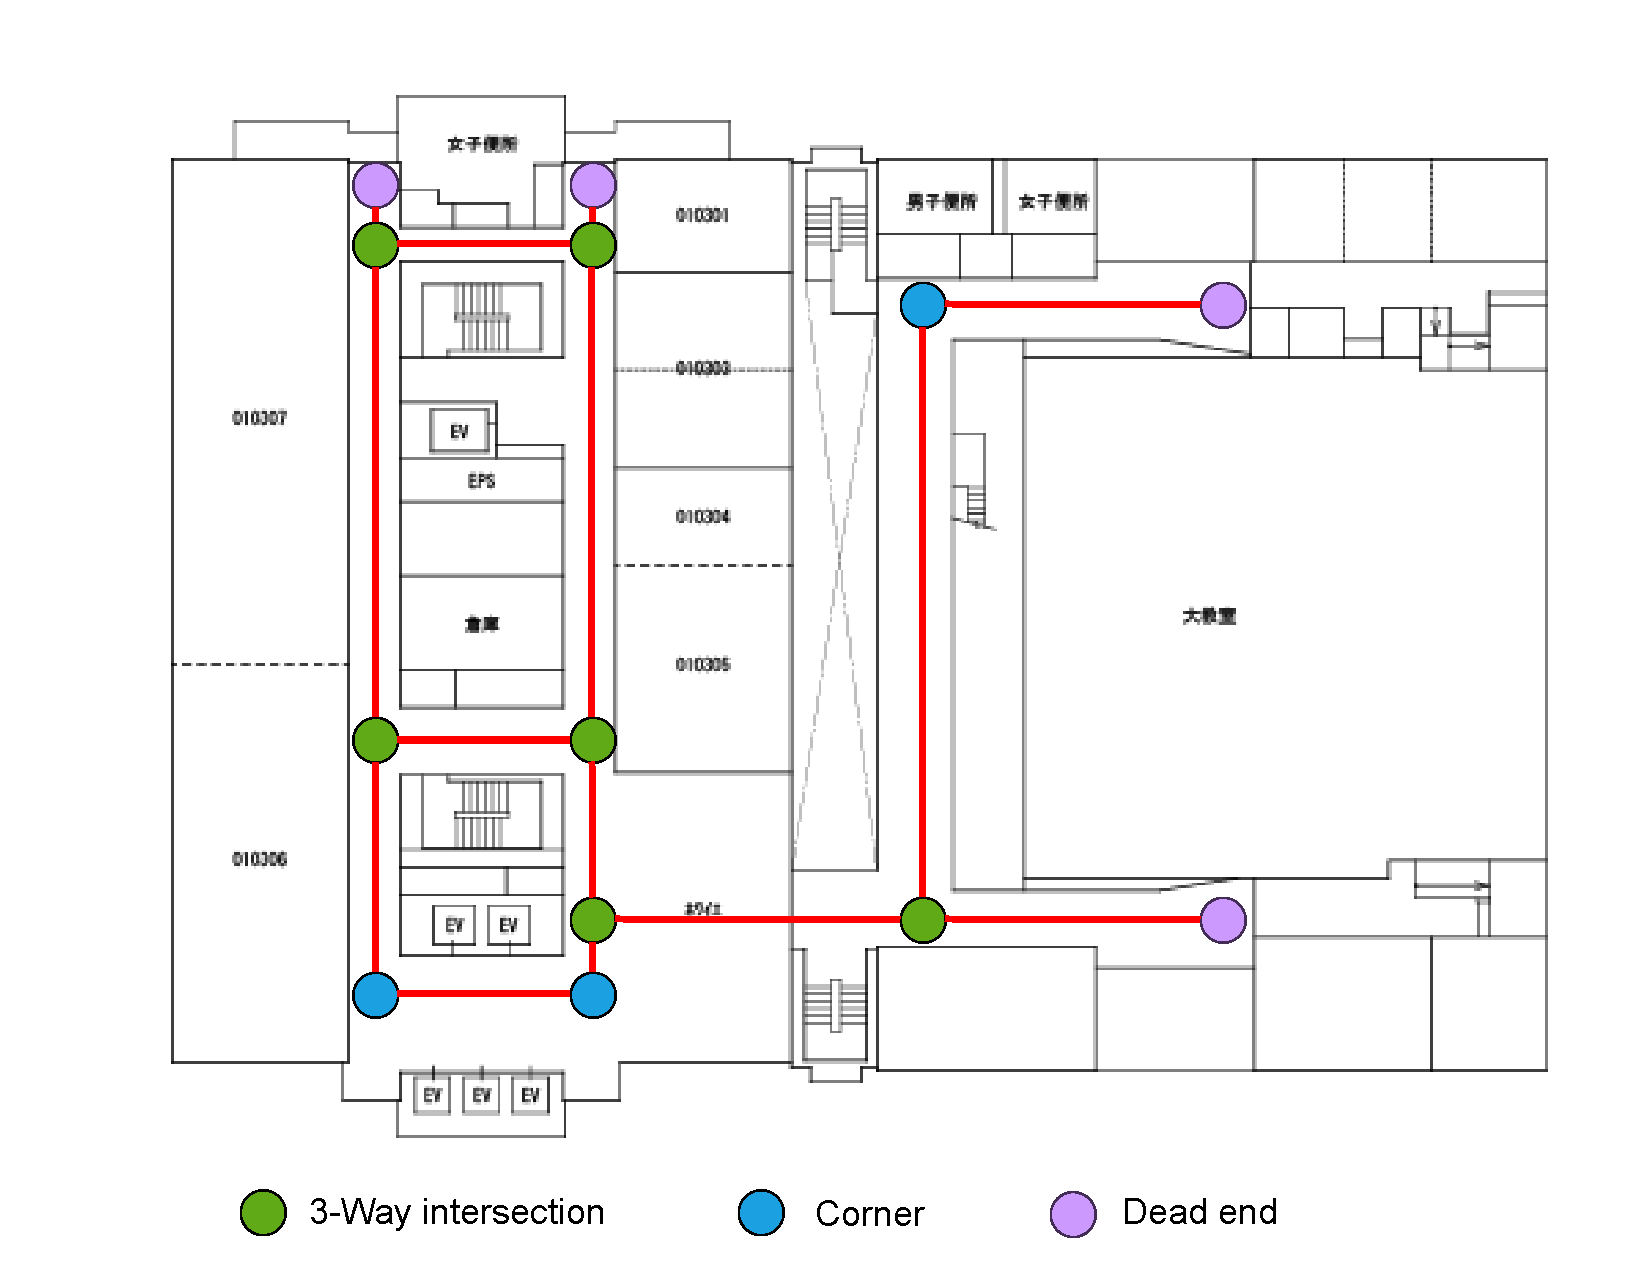
\includegraphics[width=130mm]{images/pdf/ishiguro/topo.pdf}
  \caption{Experimental environment}
  \label{fig:topo}
\end{figure}

\begin{figure}
  \centering
  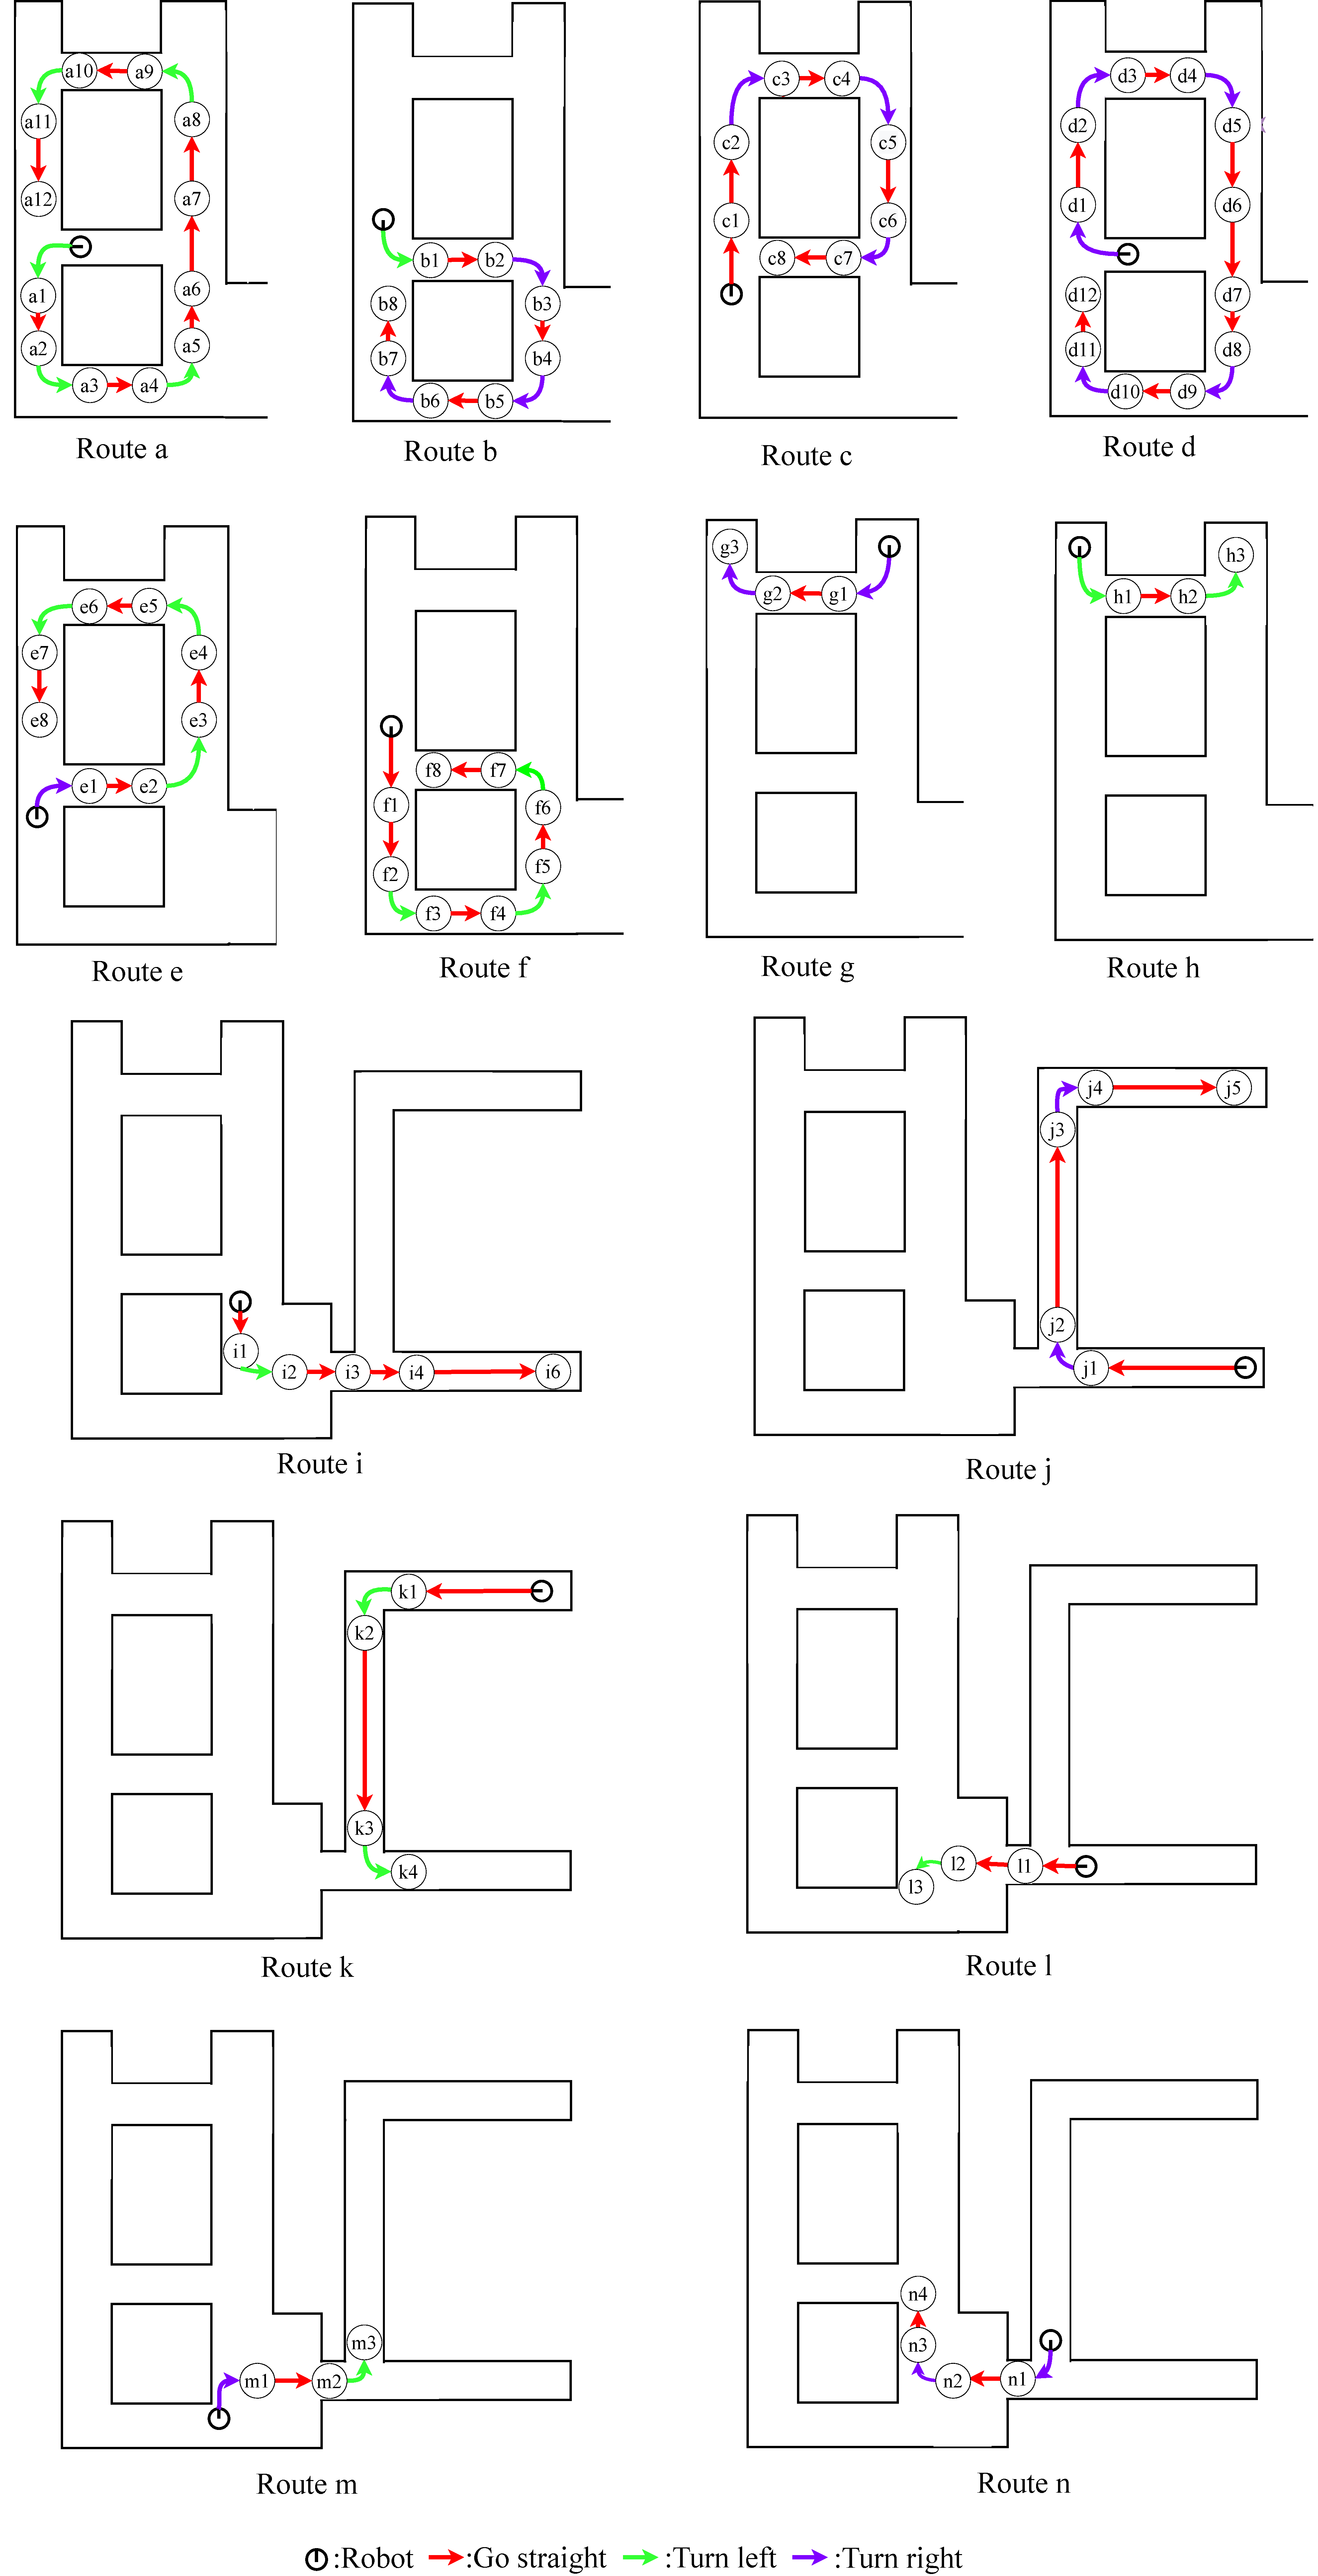
\includegraphics[width=110mm]{images/pdf/ishiguro/route.pdf}
  \caption{Experimental route}
  \label{fig:route}
\end{figure}

\newpage
\subsection{シナリオの選定}
実験では島田ら用いた50例の中から,28例を選定した.
選定するにあたって,以下の条件を設定した.

\begin{enumerate}
  \item [1)] ロボットの移動に安全性が確保できない,\figref{fig:keepout}上部に示す部分を走行ルートに含まれないこと.
  \item [2)] 経路追従モジュールができない,「後ろを向く」などその場での旋回が含まれていないこと.
  \item [3)] 正面の単眼カメラの情報のみでは通路の分類が困難な\figref{fig:keepout}下部に示す部分が走行ルートが含まれないこと.
\end{enumerate}
 
\begin{figure}
  \centering
  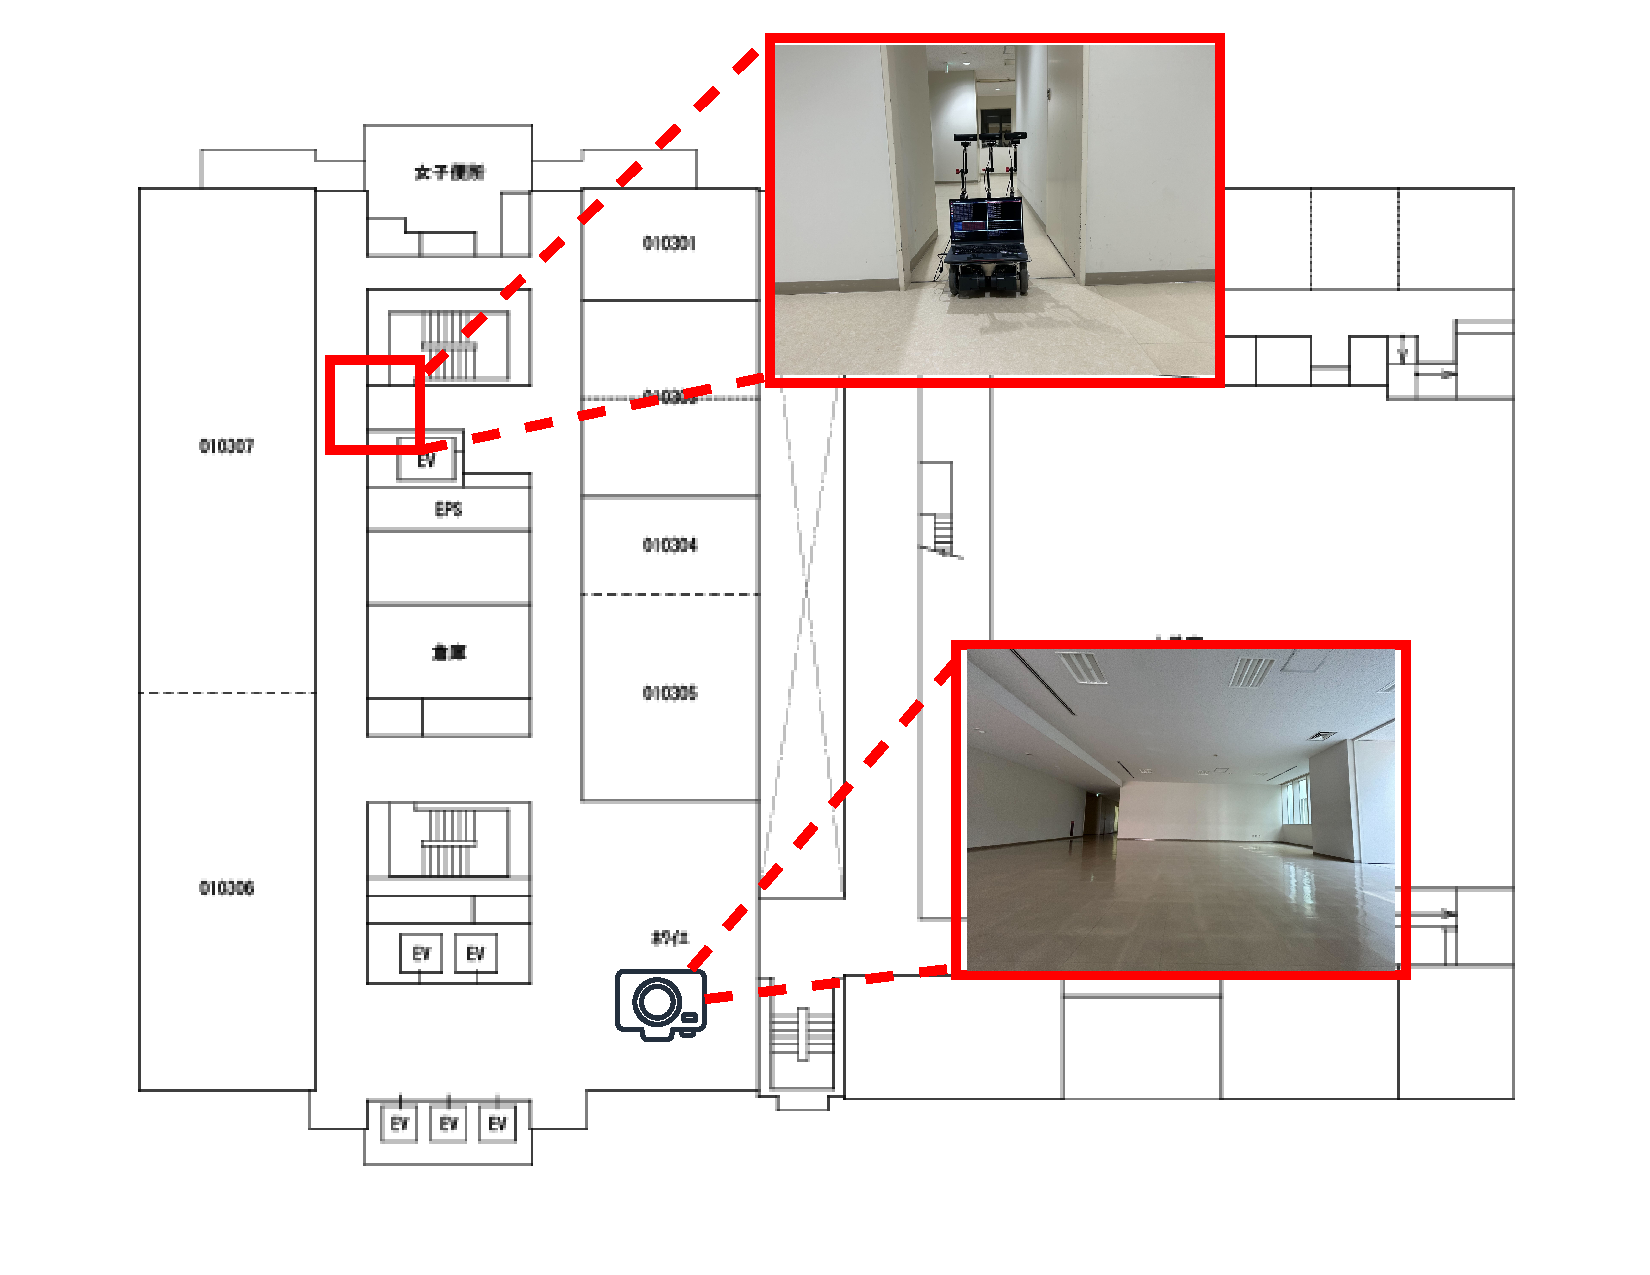
\includegraphics[width=130mm]{images/pdf/ishiguro/keepout.pdf}
  \caption{Experimenta}
  \label{fig:keepout}
\end{figure}

\clearpage
\subsection{経路追従モジュールの訓練}
\figref{fig:route}に示すルートをオンライン学習させながら 1 週走行する.
データセットの収集には藤原ら\cite{fujiwara2023}が提案する手法を用いる.
また,オンライン学習で作成したモデルに追加でオフライン学習を行う.
オフライン学習時のデータセットにはオンライン学習の際に作成したルート 1 週分のデータを用いる.
データセットからはオンライン学習と同様のバッチサイズ 8 でデータをランダムに取得し,epoch数は 20 とした.

\subsection{通路分類モジュールの訓練}
\figref{fig:route}に示すルートをROS の navigation パッケージを使用して,経路を 1 周する.
その際, 3 つのカメラからそれぞれ画像データを収集しながら走行する.
学習時のパラメータとして,バッチサイズを 32 ,epoch数を 30 とし,コストアプローチに用いた重みは\ref{tab:cost}に示す.

\begin{table}[htbp]
  \centering
  \caption{The weights assigned to each class in the experiment}\label{tab:cost}
  \begin{tabular}{c|c}
  \hline
  Class & Class weights\\
  \hline
  直進   & 1\\
  突き当たり   & 39.5\\
  角(右) & 14\\
  角(左)& 14.2 \\
  十字路 & 1  \\
  三叉路(右)& 6.6  \\
  三叉路(中央)& 7.0  \\
  三叉路(左) & 6.4  \\
  \hline
  \end{tabular}
\end{table}

\clearpage
\subsection{シナリオに基づくナビゲーション}
2 つのモジュールを訓練後,ロボットが目的地まで到達できるか確認する.
実験では,ロボットをシナリオのスタート地点,向きに配置し,シナリオを 1 例ずつ投入する.
途中で壁に衝突や,経路の選択を誤ることなく自律移動し,目的地で停止した際に成功とする.